% $Id: VM_desc.tex,v 1.4 2004/05/22 02:48:13 theurich Exp $

The {\tt ESMF\_VM} (virtual machine) class can be viewed as a generic representation of hardware and system software resources. There is exactly one VM object associated with each component in an ESMF application. The VM object handles all resource management tasks of a component and provides a topological description of the underlying configuration of the compute resources used by the component. The basic elements of a VM are called PETs, which stands for Persistent Execution Threads, and are equivalent to OS threads with a lifetime of at least that of the associated component. All VM functionality is expressed in terms of PETs. In the single-threaded case --- the only one currently accessible in ESMF --- a PET is equivalent to an MPI process. 

The resource management functions of the VM class come into play when a component creates sub--components. There are two parts to resource management, the parent and the child. When the parent component creates a child component it provides its own VM object to the {\tt ESMF\_GridCompCreate()} or {\tt ESMF\_CplCompCreate()} method and optionally specifies a {\tt petList} to limit the resources it wants to give to the child. The child on the other hand may specify during its SetServices method how it wants the inherited resources to be arranged in its own VM. Besides the SetServices method all other registered component methods will henceforth be instantiated using the thus defined child VM.

In addition to resource management and topological description the VM class offers the lowest level of ESMF communication methods. Data references in VM communication calls must be provided in raw, language specific, one-dimensional, contiguous data arrays, much like in MPI. In fact, the similarity between VM and MPI communication calls is striking and there are many equivalent point-to-point and collective communication calls. However, two major differences sets VM communication apart from its MPI counterpart. First, the transparent VM communication calls hide an array of very specific implementations, ranging from intra--process communication within multi--threaded processes, shared memory communication between processes within the same single system image, to the use of specific hardware libraries associated with the interconnection fabric in distributed systems. Second, contrary to MPI, the VM class provides non--blocking collective communication calls in addition to the non--blocking point-to-point primitives.

%\begin{center}
%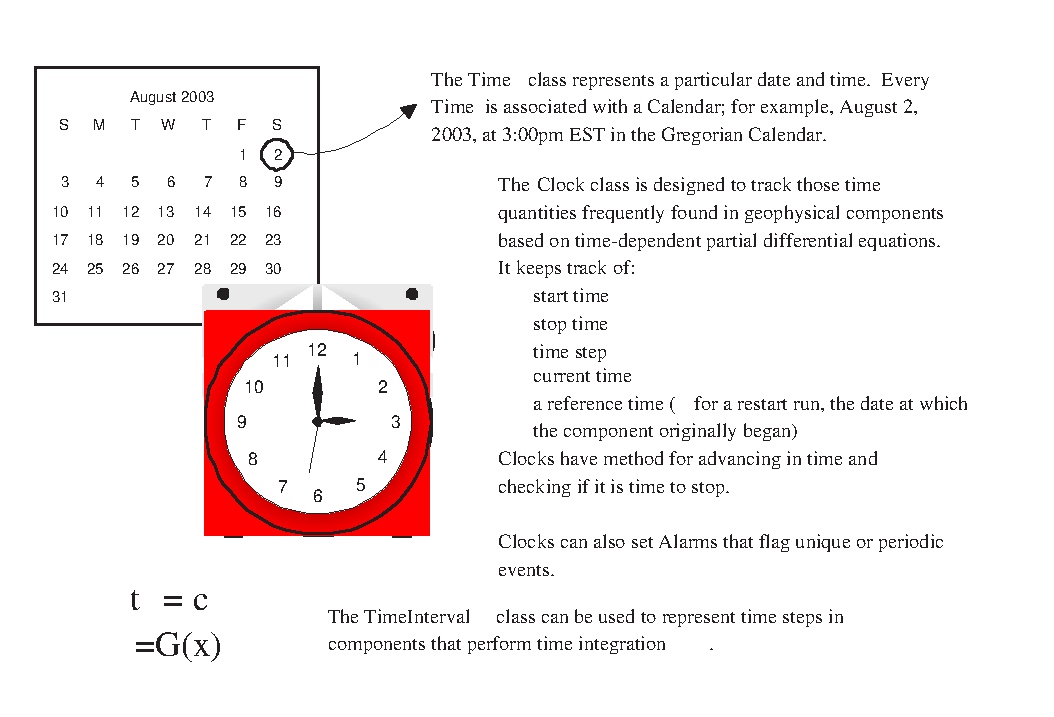
\includegraphics{TimeMgr_desc.eps}
%\end{center}
